\documentclass[handout]{beamer}

\usepackage{Haust2016glærur}

\title{Tölvunarfræði 1a}
\subtitle{Vika 12, seinni fyrirlestur}

\begin{document}

\begin{frame}
\titlepage
\end{frame}

\section{Inngangur}

\begin{frame}{Í síðasta þætti\ldots}
\begin{itemize}
 \item Teikning skoðuð betur
 \item Hreyfimyndir
 \item Óvissubil (utan bókar)
 \item Þrívíddarteikningar 
\end{itemize}
\end{frame}

\begin{frame}[fragile]{Að teikna hæðarlínur}
Viðbót við þrívíddarteikningar: 

Hægt er að teikna hæðarlínur á mjög svipaðan hátt og yfirborð eru teiknuð með \texttt{mesh} eða \texttt{surf}. Notum einfaldlega \texttt{contour} eða \texttt{contour3} í staðinn.

\begin{minted}{matlab}
>> [x,y] = meshgrid(linspace(-2,2),linspace(-2,2));
>> z = sin(x).*exp(y);
>> contour(x,y,z)
\end{minted}

\end{frame}

\section{Litavarpanir}

\begin{frame}[fragile]{Litavarpanir}
\begin{columns}
\column{0.5\textwidth}
\begin{itemize}
 \item Við höfum séð að mörg teikniföll eru með sjálfgefna liti
 \item Þessum sjálfgefnu litum má breyta með því að stilla litavörpun (e. \emph{colormap}) fyrir teikninguna
\begin{minted}{matlab}
>> colormap('nafn vörpunar')
\end{minted}
\end{itemize}
\column{0.5\textwidth}
\begin{itemize}
 \item Nokkrar innbyggðar litavarpanir:
 \begin{itemize}
  \item parula
  \item jet
  \item hsv
  \item hot
  \item cool
  \item spring
  \item summer
  \item autumn
  \item winter
  \item gray
  \item bone
  \item copper
  \item pink
 \end{itemize}
\end{itemize}
\end{columns}
\end{frame}

\begin{frame}[fragile]{Litavarpanir}
\begin{itemize}
 \item Litavörpun er talnafylki með þremur dálkum
 \item Hver lína táknar einn RGB-lit
 \begin{itemize}
  \item Hver tala er á bilinu 0 til 1 og táknar hlutfall viðkomandi grunnlits
 \end{itemize}
 \item Við getum skilgreint okkar eigin litavarpanir!
 \item Svart-hvítar rendur:
\end{itemize}
\begin{minted}{matlab}
>> myMap = repmat([0 0 0;1 1 1],4,1);
>> colormap(myMap)
\end{minted}
\end{frame}

\begin{frame}{Hráar myndir}
\begin{itemize}
 \item Við getum teiknað upp talnafylki með \texttt{image} fallinu
 \begin{itemize}
  \item Hvert stak í fylkinu er teiknað upp sem ferningur
  \item Gildi stakanna er notað til að vísa í litavörpun
 \end{itemize}
 \item Við getum líka fengið hráa mynd með því að nota \texttt{imagesc} fallið, en þá eru litirnir skalaðir til hlutfallslega
\end{itemize}

\end{frame}


\section{Teiknihandföng}

\begin{frame}{Teiknihandföng}
\begin{itemize}
 \item Allar teikningar í Matlab samanstanda af teiknihlutum (e. \emph{graphics objects})
 \begin{itemize}
  \item Vísa má í teiknihluti með handföngum (e. \emph{handles})
  \item Handfang vísar einkvæmt í hlutinn
 \end{itemize}
 \item Teiknihlutir eru af ýmsum gerðum
 \begin{itemize}
  \item Ásar, línur, texti, \ldots
  \item Þessir hlutir hafa mismunandi eiginleika
 \end{itemize}
\end{itemize}
\end{frame}

\begin{frame}[fragile]{Plot objects}
Teikniföllin (\texttt{plot}, \texttt{bar}, \texttt{pie}) skila handfangi fyrir teiknihlutinn
\begin{minted}{matlab}
>> x = -2*pi : 0.1 : 2*pi;
>> y = sin(x);
>> handle = plot(x,y)
handle = 
  Line with properties:
  ...
\end{minted}
\end{frame}

\begin{frame}[fragile]{Eiginleikar teiknihluta}
\begin{itemize}
 \item Upprifjun: Getum náð í gildi einstakra eiginleika með \texttt{get}
 \begin{minted}{matlab}
 >> get(handle)
  AlignVertexCenters: 'off'
  ...
 \end{minted}
 \item Getum breytt gildum eiginleika með \texttt{set}
 \begin{minted}{matlab}
 >> set(handle, 'LineWidth', 2.5)
 \end{minted}
 \item Einnig er hægt að setja þá í upphaflegu teikniskipunina
 \begin{minted}{matlab}
 >> handle= plot(x,y,'LineWidth', 2.5);
 \end{minted}
\end{itemize}
\end{frame}

\section{Grunnhlutir}

\begin{frame}[fragile]{Core objects}
\begin{itemize}
 \item Matlab er með ákveðna grunnhluti (e. \emph{core objects}) til teiknunar
 \begin{itemize}
  \item Lína (\texttt{line}), texti (\texttt{text}), rétthyrningur (\texttt{rectangle})
 \end{itemize}
 \item Hægt er að teikna þá með innbyggðum föllum
\begin{minted}{matlab}
>> h1 = line([3 1], [2 4], 'Color', 'r');
\end{minted}
\end{itemize}
\end{frame}

\begin{frame}{Línur}
\begin{itemize}
 \item Línur eru kunnuglegur teiknihlutur
 \begin{itemize}
  \item \texttt{plot} fallið býr til línur
 \end{itemize}
 \item Línur hafa ýmsa eiginleika
 \begin{itemize}
  \item \texttt{LineStyle} - heil lína, punktalína, engin lína
  \item \texttt{LineWidth} - þykkt línunnar
  \item \texttt{Marker} - hvaða tákn á að sýna í gagnapunktum
 \end{itemize}
\end{itemize}
\end{frame}

\begin{frame}[fragile]{Texti}
\begin{itemize}
 \item Fallið \texttt{text} setur texta inn á teikninguna
 \begin{itemize}
  \item Almennt snið: \texttt{text(x,y,'strengur')}
  \item \texttt{x} og \texttt{y} eru staðsetning neðra vinstra horns textakassans
 \end{itemize}
 \item Hægt er að nota sumar \LaTeX-skipanir í strengnum
 \begin{itemize}
  \item Líka í föllum eins og \texttt{title} og \texttt{xlabel}
 \end{itemize}
\end{itemize}

\begin{minted}{matlab}
>> x = 0:0.01:5;
>> y = exp(x);
>> line(x,y,'LineWidth',3);
>> textHandle = text(3,50,'e^x \rightarrow');
>> set(textHandle, 'Fontsize', 20);
\end{minted}

\end{frame}

\begin{frame}{Texti}
\begin{center}
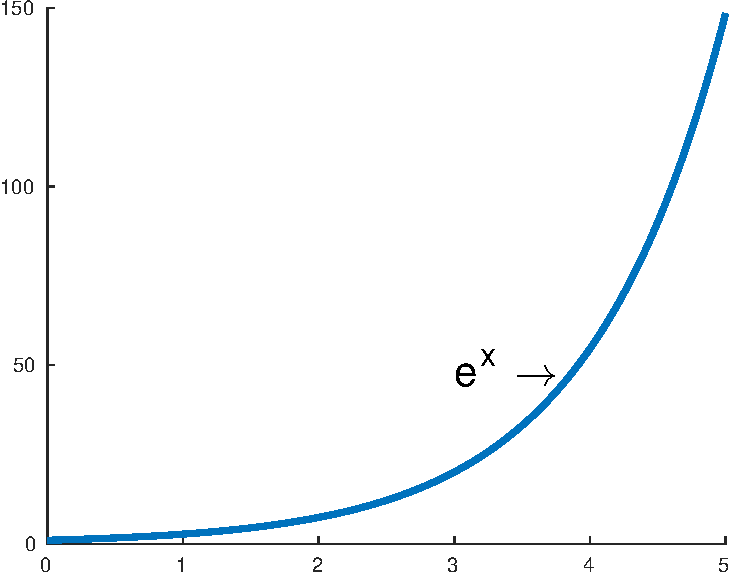
\includegraphics[width=0.8\textwidth]{Pics/exp-label}
\end{center}
\end{frame}

\begin{frame}[fragile]{Rétthyrningar}
\begin{itemize}
 \item Fallið \texttt{rectangle} teiknar rétthyrning
 \begin{itemize}
  \item Staðsetning (\texttt{Position}) hans er gefin með \texttt{[x, y, w, h]}
  \begin{itemize}
   \item Staðsetning vinstra neðra horns, breidd og hæð
  \end{itemize}
 \end{itemize}
 \item Sveigja (\texttt{Curvature}) hans er tveggja staka vigur með gildi frá \texttt{[0,0]} til \texttt{[1,1]}
 \begin{itemize}
  \item Fyrra gildið er hversu hátt hlutfall af láréttu línunum er sveigt, hið seinna á við lóðréttu línurnar
 \end{itemize}
\end{itemize}
\begin{minted}{matlab}
>> rectangleHandle = rectangle('Position', [2 1 4 2]);
>> axis([0 8 0 4])
>> set(rectangleHandle, 'Curvature', [0.2 0.2])
\end{minted}

\end{frame}

\begin{frame}{Rétthyrningar}
\begin{center}
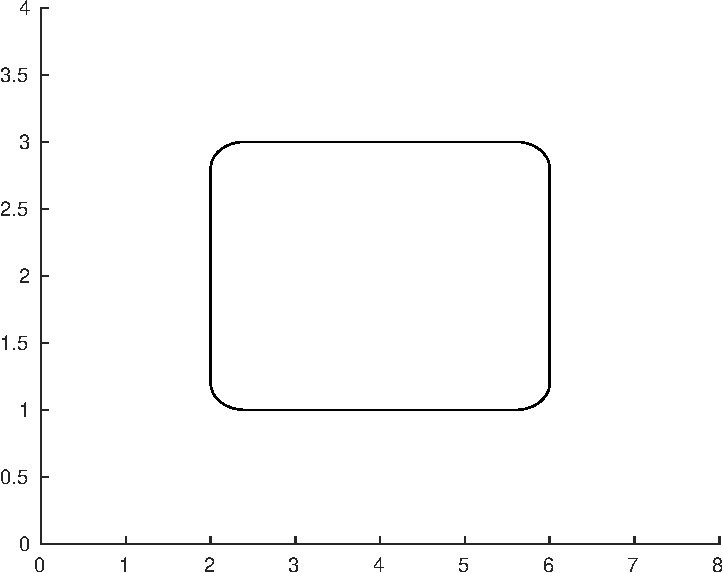
\includegraphics[width=0.8\textwidth]{Pics/rectangle-example}
\end{center}
\end{frame}

\begin{frame}[fragile]{Hringir}
\pause
\begin{itemize}
 \item Hægt er að teikna hringi og sporöskjur með því að búa til ``rétthyrninga'' með sveigjuna \texttt{[1 1]}
\end{itemize}
\begin{minted}{matlab}
>> circleHandle = rectangle('Curvature',[1 1]);
>> axis('square')
>> axis([-1 2 -1 2])
\end{minted}
\end{frame}

\begin{frame}{Hringir}
\begin{center}
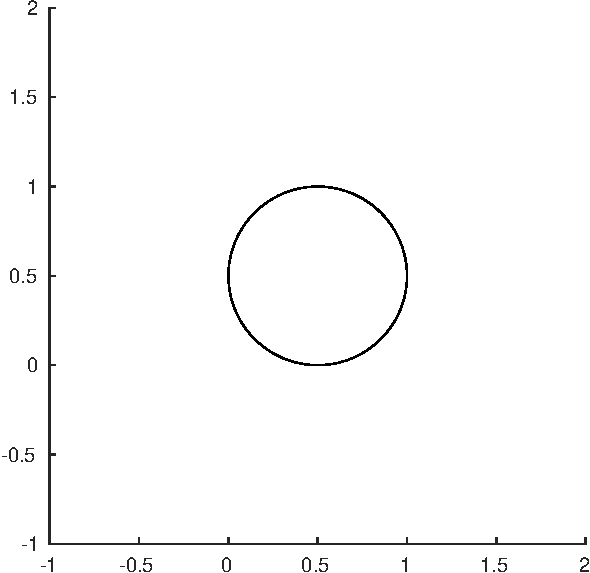
\includegraphics[width=0.6\textwidth]{Pics/circle-example}
\end{center}
\end{frame}

\begin{frame}[fragile]{Marghyrningar}
\begin{columns}
\column{0.5\textwidth}
\begin{itemize}
 \item Til að teikna marghyrninga má nota fallið \texttt{patch}
 \begin{itemize}
  \item Fær inn $x$ og $y$ hnit
 \end{itemize}
\end{itemize}
\begin{minted}{matlab}
>> xCoords = [1 4 3 2];
>> yCoords = [1 1 2 2];
>> patch(xCoords,yCoords,'r')
>> axis([0 5 0 3])
\end{minted}
\column{0.5\textwidth}
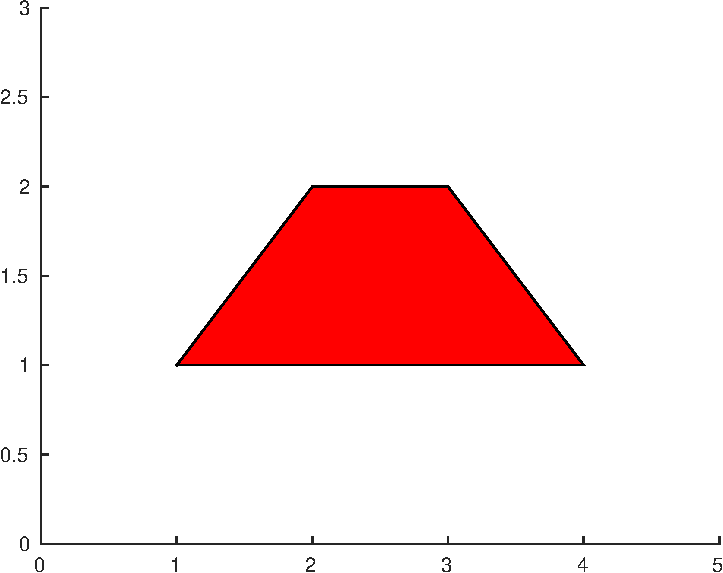
\includegraphics[width=\textwidth]{Pics/patch-example}
\end{columns}
\end{frame}


\begin{frame}{Fyrirlestraræfing}
\begin{columns}
\column{0.5\textwidth}
Skráið ykkur inn á \url{http://socrative.com/} og klárið æfinguna.

Herbergisnúmer = \texttt{TOL105G2016}

Notendanafn = HÍ-tölvupóstfang
\column{0.5\textwidth}
\begin{center}
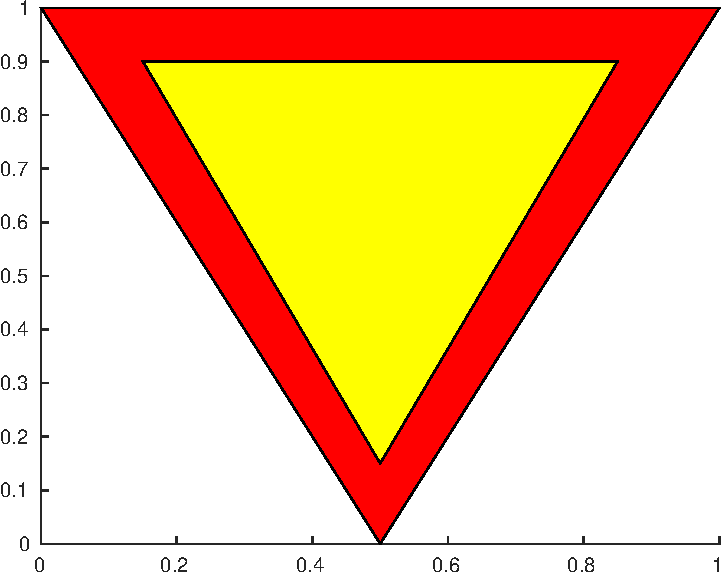
\includegraphics[width=0.8\linewidth]{Pics/bidskylda}
\end{center}
\end{columns}
\end{frame}



\end{document}
